\documentclass{article}
\usepackage{amsmath} % Requerido para elementos matemáticos
\usepackage[utf8]{inputenc}			
\usepackage[spanish, es-tabla]{babel} %Ajustar idioma: español
\spanishdecimal{.}
\usepackage{graphicx} % Requerido para la inclusión de imágenes
%\usepackage{natbib} % Requerido para el cambio de formato a formato APA
\usepackage{lipsum}

\author{David Silva}
\date{\today}
\title{Referencias bibliográficas}
\begin{document}
	\maketitle
	\vspace{2cm}
	\begin{center}
		
\includegraphics[width=6cm]{img/logo}
	\end{center}

	\newpage
	\tableofcontents
	
	\newpage
	\section{Introducción}
	\lipsum[1-4]
	\subsection{Marco teórico}
	\lipsum[1-2]
	\subsection{Demostraciones}
	\lipsum[1]
	
	Tal como se muestra en la siguiente ecuación:
	\begin{equation}
		\phi (x,t) = A sin (\omega t - kx)
		\label{eq:Onda}
	\end{equation}
	
	
	\section{Desarrollo}
	\lipsum[3-5]
	\subsection{Mediciones}
	\lipsum[1-2]
	
	\lipsum[3-4]
	\subsection{Evidencia fotográfica}
	
	\begin{figure}[h]
		\centering
		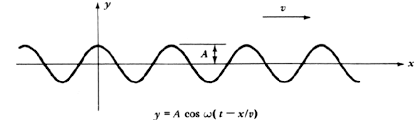
\includegraphics[width=8cm, height=5cm]{img/onda}
		\label{fig:Onda}
		\caption{Comportamiento de una onda armónica senoidal.}
	\end{figure}
		
	
	\subsection{Cálculos}
	
	\begin{table}
		\centering
		\begin{tabular}{cc}
			\hline
			Parámetro & Repetición 1\\
			\hline
			A & 5\\
			$\omega$ & 5\\
			k & 8\\		
		\end{tabular}
	
	\caption{Valores obtenidos experimentalmente}
	\label{tab:exp}
	\end{table}

	
	Tal como se dedujo en la demostración \eqref{eq:Onda} podremos determinar la naturaleza de una onda sustituyendo los valores en la ecuación por los registrados en la tabla \ref{tab:exp}.
	$$
	\phi (x,t) = 5 sin (5t - 8x)
	$$
	\newpage
	\section{Conclusiones}
	\lipsum[1]
	
	\bibliography{bib/biblio}
	\bibliographystyle{apalike}
	
\end{document}
